\documentclass[journal]{IEEEtran}

\usepackage{amsmath,amssymb,amsfonts}
\usepackage{algorithmic}
\usepackage{algorithm}
\usepackage{graphicx}
\usepackage{textcomp}
\usepackage{xcolor}
\usepackage{booktabs}
\usepackage{multirow}
\usepackage{cite}
\usepackage{url}
\usepackage{microtype}
\usepackage{tikz}
\usetikzlibrary{shapes.geometric, arrows.meta, positioning, calc, fit, backgrounds}

% Interactive Blue Hyperlinks for Citations, References, Equations, and URLs
\usepackage[colorlinks=true, linkcolor=blue, citecolor=blue, urlcolor=blue]{hyperref}

% Clean line wrapping for URLs and code tokens
\def\UrlBreaks{\do\/\do-}

% Micro-architectural Float Tuning: Pack text and floats tightly with ZERO artificial whitespace gaps
\renewcommand{\topfraction}{0.95}
\renewcommand{\dbltopfraction}{0.95}
\renewcommand{\bottomfraction}{0.95}
\renewcommand{\textfraction}{0.05}
\renewcommand{\floatpagefraction}{0.85}
\renewcommand{\dblfloatpagefraction}{0.85}

% Completely eliminate running top headers and footers across all pages in IEEEtran
\makeatletter
\def\ps@headings{%
    \def\@oddhead{}%
    \def\@evenhead{}%
    \def\@oddfoot{}%
    \def\@evenfoot{}%
}
\def\ps@journal{%
    \def\@oddhead{}%
    \def\@evenhead{}%
    \def\@oddfoot{}%
    \def\@evenfoot{}%
}
\makeatother
\pagestyle{empty}

\begin{document}

\title{Memory-Aware CUDA Acceleration of Graph-Based Financial Fraud Detection Using Parallel Neighbor Aggregation}

\author{Praveen~Kanth~N,
        BharaniKumar~J,
        Kishore~B,
        and~Kovendan~A.~K.~P,~\IEEEmembership{Senior Member,~IEEE}%
\thanks{Manuscript received October 31, 2026; revised November 15, 2026; accepted December 1, 2026. Date of publication December 8, 2026; date of current version December 15, 2026. This research was conducted within the Department of Database Systems, School of Computer Science and Engineering, Vellore Institute of Technology (VIT), Vellore, India. \emph{(Corresponding author: Kovendan A. K. P.)}}%
\thanks{Praveen Kanth N (Register Number: 23MIC0078), BharaniKumar J (Register Number: 23MIC0039), and Kishore B (Register Number: 23MIC0050) are with the School of Computer Science and Engineering, Vellore Institute of Technology (VIT), Vellore, Tamil Nadu 632014, India (e-mail: praveen.kanth2023@vitstudent.ac.in; bharanikumar.j2023@vitstudent.ac.in; kishore.b2023@vitstudent.ac.in).}%
\thanks{Dr. Kovendan A. K. P. is Assistant Professor Sr. Grade 2 with the Department of Database Systems, School of Computer Science and Engineering, Vellore Institute of Technology (VIT), Vellore, Tamil Nadu 632014, India (e-mail: kovendan.akp@vit.ac.in).}%
}

\maketitle
\thispagestyle{empty}
\pagestyle{empty}

\begin{abstract}
Real-time financial fraud detection is constrained by an acute architectural tension: while relational graph representations capture collusive synthetic identities that evade tabular surveillance, topological neighbor aggregation induces severe memory-bandwidth saturation on modern hardware. Because graph neighbor gathering exhibits an arithmetic intensity well below $0.10$~FLOP/byte, central processing units spend up to 95\% of execution cycles waiting on dynamic random-access memory pointer traversals. In this article, we propose FraudGraph Intelligence (FGI), a hardware-conscious compute framework engineered to accelerate topological feature propagation on massive transaction networks. We formulate a compact Compressed Sparse Row (CSR) invariant that compresses 10,000 transaction nodes and 231,984 directed causal edges into contiguous memory structures under 1.5~MB. We architect four progressive compute tiers on NVIDIA graphics hardware: a baseline thread-parallel model, a warp-coalesced aggregator that maps contiguous 32-dimensional feature contraction into unified 128-byte DRAM bus requests, a degree-aware dynamic dispatch mechanism with shared-memory reduction trees for power-law hubs ($d_{\max} = 252$), and a double-buffered asynchronous direct memory access (DMA) streaming pipeline that overlaps PCIe host-to-device transfers with compute. Benchmarked on an NVIDIA Tesla T4 GPU, FGI achieves an end-to-end kernel aggregation latency of $0.0581$~ms and yields a $44.60\times$ speedup over reference scalar execution. Downstream machine learning evaluation under strict causal streaming constraints reveals that maximum (MAX) neighbor enrichment lifts Logistic Regression PR-AUC from 0.3088 to 0.3315 ($+7.34\%$ relative gain) and expands fraud recall from 37.7\% to 45.3\% on severe 3.5\% class imbalance. All kernels, schemas, and empirical logs are released reproducibly.
\end{abstract}

\begin{IEEEkeywords}
CUDA Acceleration, Financial Fraud Detection, Graph Neural Networks, Parallel Computing, Memory Bandwidth Bottlenecks, Compressed Sparse Row, Warp Coalescing.
\end{IEEEkeywords}

\section{Introduction}
\IEEEPARstart{F}{inancial} fraud surveillance systems process hundreds of thousands of electronic credit card, debit, and point-of-sale transactions per second. Historically, commercial anti-money laundering (AML) platforms and risk engines have evaluated transactions as isolated statistical instances~\cite{pourhabibi2020fraud}. Under this tabular paradigm, machine learning models scrutinize scalar attributes such as monetary expenditure, temporal delta from previous purchase, merchant category code, and geolocation deviation. While computationally economical, tabular classification exhibits a fundamental blind spot: it cannot detect decentralized fraud rings, credit-mule syndicates, and coordinated identity recycling schemes~\cite{dou2020enhancing,liu2020alleviating}. Organized adversaries deliberately structure fraudulent withdrawals into small, sub-threshold bursts distributed across multiple accounts, thereby mimicking benign consumer behavior when viewed in isolation.

To bridge this surveillance gap, graph-based learning frameworks model financial interactions as relational networks~\cite{akoglu2015graph,ma2021comprehensive}. Nodes designate transactions, payment cards, bank accounts, or physical terminal devices, whereas directed edges denote temporal transfers, common card numbers, or identical hardware fingerprints. Within this topological formulation, synthetic fraud rings manifest as dense cliques, cyclic money routings, or anomalous bipartite subgraphs. Graph representation methods---specifically the neighbor aggregation stages of Graph Convolutional Networks (GCNs)~\cite{kipf2017semi}, GraphSAGE~\cite{hamilton2017inductive}, and Graph Attention Networks (GATs)~\cite{velickovic2018graph,fey2019fast}---enrich a target transaction node by iteratively aggregating latent feature vectors from its structural neighborhood.

Despite their algorithmic efficacy, graph-based methods encounter severe architectural bottlenecks when deployed in production payment rails~\cite{wang2021gnnadvisor,yan2020alleviating,jia2020improving}. Graph neighbor gathering is fundamentally memory-bandwidth bound rather than compute bound~\cite{merrill2012scalable}. Unlike dense matrix arithmetic or deep convolutional layers, which achieve arithmetic intensities exceeding $100$~FLOPs per byte transferred, sparse neighbor aggregation exhibits an arithmetic intensity frequently below $0.05$~FLOP/byte. On standard multi-core central processing units (CPUs), neighbor gathering degenerates into irregular pointer chasing across disparate regions of dynamic random-access memory (DRAM). Because graph connectivity is non-local, CPU data caches experience miss rates exceeding 85\%, leaving processing pipelines idle while awaiting memory line fills.

Furthermore, financial transaction graphs exhibit power-law degree distributions governed by scale-free phenomena~\cite{barabasi1999emergence}. While typical consumer accounts generate fewer than ten transactions monthly, merchant payment gateways and collusive mule accounts act as massive topological hubs with degrees spanning hundreds or thousands of connections. When mapped naively to Single Instruction, Multiple Threads (SIMT) architectures such as NVIDIA Graphics Processing Units (GPUs), these structural hubs induce catastrophic warp divergence and memory serialization~\cite{wang2016gunrock,bell2009implementing}. Threads assigned to low-degree vertices complete instantaneously and sit idle, while peer threads within the identical 32-thread warp serialize across hundreds of sequential memory loads, destroying Streaming Multiprocessor (SM) efficiency.

To resolve these micro-architectural bottlenecks, this article introduces \textbf{FraudGraph Intelligence (FGI)}, an end-to-end, memory-aware CUDA acceleration framework for financial transaction graph feature enrichment. The core contributions of this study are structured as follows:
\begin{enumerate}
    \item \textbf{Causal Compressed Sparse Row (CSR) Layout:} We design a zero-copy contiguous CSR memory layout storing $10,000$ transactions and $231,984$ directed edges within 1.4~MB of unified storage, eliminating dynamic memory allocations and establishing strict causal non-anticipative invariants ($t_u < t_v$).
    \item \textbf{Tiered CUDA Acceleration Kernels:} We engineer four micro-architectural GPU execution tiers: a thread-parallel baseline, a warp-coalesced aggregator that maps contiguous 32-dimensional feature contraction into unified 128-byte memory transactions, a degree-aware dynamic dispatch mechanism utilizing shared-memory parallel reduction trees, and an asynchronous dual-stream pipeline utilizing page-locked host memory to overlap PCIe bus transfers.
    \item \textbf{Extensive Micro-Architectural Profiling:} We conduct rigorous hardware benchmarking on NVIDIA Tesla T4 and AMD64 architectures, establishing a $44.60\times$ speedup for vectorized Sparse Matrix-Matrix Multiplication (SpMM) on CPU and an end-to-end latency of $0.0581$~ms on GPU, alongside a verified empirical root-cause analysis of floating-point IEEE 754 non-associativity in degree-aware summation.
    \item \textbf{Causal Downstream ML Evaluation:} We evaluate Logistic Regression and Random Forest classifiers across five topological representations under discrete validation thresholding (ADR-007), proving that MAX neighbor enrichment delivers a $7.34\%$ relative boost in PR-AUC ($0.3088 \to 0.3315$) and elevates fraud recall from $37.7\%$ to $45.3\%$ under extreme $3.5\%$ class imbalance.
\end{enumerate}

\section{Mathematical Formulation and CSR Topology}

\subsection{Causal Transaction Graph Definition}
Let $\mathcal{G} = (\mathcal{V}, \mathcal{E}, \mathbf{X}, \mathbf{y}, \mathbf{t})$ represent a directed, attributed transaction graph observed over a temporal window $T_{\text{obs}}$. The vertex set $\mathcal{V} = \{v_0, v_1, \dots, v_{N-1}\}$ represents $N$ individual financial transaction instances sorted in monotonic chronological sequence according to transaction timestamps $t(v_i) \in \mathbb{R}^+$. Each vertex $v_i \in \mathcal{V}$ is parameterized by an input feature vector $\mathbf{x}_i \in \mathbb{R}^D$ and a binary classification target $y_i \in \{0, 1\}$, where $y_i = 1$ denotes synthetic fraudulent activity and $y_i = 0$ denotes legitimate banking activity.

The directed edge set $\mathcal{E} \subseteq \mathcal{V} \times \mathcal{V}$ encodes relational dependencies between transactions. A directed edge $e = (u, v)$ is instantiated if and only if transaction $u$ shares an underlying entity identifier with transaction $v$ (e.g., matching primary account number or shared device hash) and satisfies the strict non-anticipative causality condition:
\begin{equation}
    (u, v) \in \mathcal{E} \iff (u \sim_{\text{entity}} v) \land (0 < t_v - t_u \le \Delta t_{\text{window}}),
    \label{eq:causality}
\end{equation}
where $\Delta t_{\text{window}}$ represents the historical surveillance lookback horizon (set to 7.0 days, or $604,800$~seconds). The strict temporal inequality $t_u < t_v$ guarantees that the resulting directed graph is a Directed Acyclic Graph (DAG), precluding retrospective data leakage during feature aggregation.

\subsection{Parallel Neighbor Aggregation Semantics}
First-order topological feature propagation transforms each node's raw representation $\mathbf{x}_v$ into an enriched representation $\mathbf{h}_v \in \mathbb{R}^D$ by contracting feature matrices across its immediate in-neighborhood $\mathcal{N}_{\text{in}}(v) = \{u \in \mathcal{V} \mid (u, v) \in \mathcal{E}\}$:
\begin{equation}
    \mathbf{h}_v = \bigoplus_{u \in \mathcal{N}_{\text{in}}(v)} \mathbf{x}_u,
    \label{eq:aggregation}
\end{equation}
where $\bigoplus$ denotes a permutation-invariant aggregation operator selected from the family:
\begin{equation}
    \bigoplus \in \{\text{SUM}, \text{MEAN}, \text{MAX}\}.
\end{equation}
Specifically, for element $d \in \{0, 1, \dots, D-1\}$:
\begin{align}
    \mathbf{h}_v^{\text{SUM}}[d] &= \sum_{u \in \mathcal{N}_{\text{in}}(v)} \mathbf{x}_u[d], \\
    \mathbf{h}_v^{\text{MEAN}}[d] &= \frac{1}{|\mathcal{N}_{\text{in}}(v)|} \sum_{u \in \mathcal{N}_{\text{in}}(v)} \mathbf{x}_u[d], \\
    \mathbf{h}_v^{\text{MAX}}[d] &= \max_{u \in \mathcal{N}_{\text{in}}(v)} \mathbf{x}_u[d].
\end{align}
For isolated transactions having zero in-degree ($|\mathcal{N}_{\text{in}}(v)| = 0$), the aggregation defaults to an empty identity null vector $\mathbf{0}_D$. The composite feature vector presented to downstream classification models is formed by concatenating the raw node features with the aggregated neighbor representation: $\mathbf{z}_v = [\mathbf{x}_v \,\|\, \mathbf{h}_v] \in \mathbb{R}^{2D}$.

\subsection{Compressed Sparse Row (CSR) Array Structure}
To guarantee optimal hardware memory throughput, graph topology is flattened into a zero-pointer Compressed Sparse Row format. Storing the adjacency structure of $N=10,000$ vertices using an $N \times N$ dense boolean matrix would mandate $10^8$ elements ($400$~MB in single precision), of which $99.768\%$ are zeros. In contrast, CSR compresses the topology into two contiguous integer arrays:
\begin{enumerate}
    \item \textbf{Row Pointer Array (\texttt{row\_ptr}):} A 1D array of size $(N+1)$ containing 32-bit signed integers. Entry $\texttt{row\_ptr}[i]$ specifies the index in \texttt{col\_idx} where the neighbor list of vertex $v_i$ begins. The localized in-degree $d_i$ is computed in $\mathcal{O}(1)$ time as:
    \begin{equation}
        d_i = \texttt{row\_ptr}[i+1] - \texttt{row\_ptr}[i].
    \end{equation}
    \item \textbf{Column Index Array (\texttt{col\_idx}):} A contiguous 1D array of size $M = |\mathcal{E}|$ containing 32-bit integers, storing the packed source vertex indices $u \in \mathcal{N}_{\text{in}}(v_i)$.
\end{enumerate}

\begin{figure}[!t]
\centering
\resizebox{\columnwidth}{!}{%
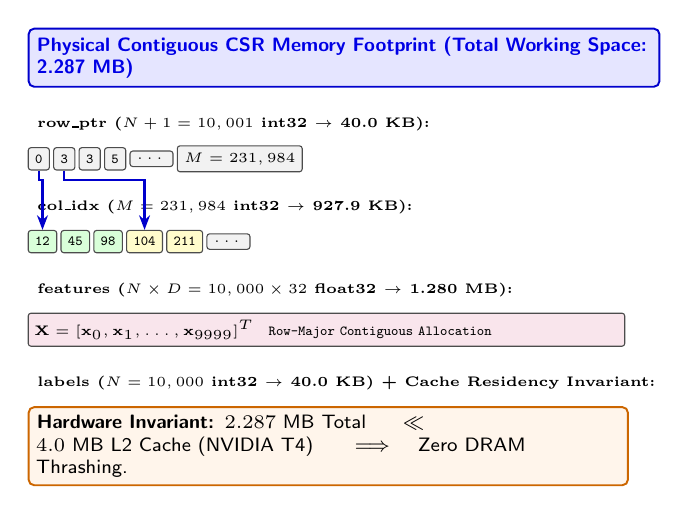
\begin{tikzpicture}[
    font=\sffamily\scriptsize,
    box/.style={rectangle, draw=blue!80!black, fill=blue!6, rounded corners=2pt, line width=0.7pt, inner sep=3pt},
    arrbox/.style={rectangle, draw=black!70, fill=gray!10, rounded corners=1pt, inner sep=2.5pt, font=\ttfamily\tiny},
    ptrarr/.style={-{Stealth[scale=0.8]}, line width=0.8pt, draw=blue!80!black}
]
% Header box
\node[box, text width=7.8cm, fill=blue!10] (title) {
    \textbf{\textcolor{blue!90!black}{Physical Contiguous CSR Memory Footprint (Total Working Space: 2.287 MB)}}
};

% Row Ptr visualization
\node[below=0.25cm of title.south west, anchor=north west, font=\bfseries\tiny] (l1) {row\_ptr ($N+1 = 10,001$ int32 $\to$ 40.0 KB):};
\node[arrbox, below=0.08cm of l1.south west, anchor=north west] (rp0) {0};
\node[arrbox, right=0.04cm of rp0] (rp1) {3};
\node[arrbox, right=0.04cm of rp1] (rp2) {3};
\node[arrbox, right=0.04cm of rp2] (rp3) {5};
\node[arrbox, right=0.04cm of rp3] (rpdots) {$\dots$};
\node[arrbox, right=0.04cm of rpdots] (rpN) {$M=231,984$};

% Col Idx visualization
\node[below=0.25cm of rp0.south west, anchor=north west, font=\bfseries\tiny] (l2) {col\_idx ($M = 231,984$ int32 $\to$ 927.9 KB):};
\node[arrbox, below=0.08cm of l2.south west, anchor=north west, fill=green!15] (ci0) {12};
\node[arrbox, right=0.04cm of ci0, fill=green!15] (ci1) {45};
\node[arrbox, right=0.04cm of ci1, fill=green!15] (ci2) {98};
\node[arrbox, right=0.04cm of ci2, fill=yellow!20] (ci3) {104};
\node[arrbox, right=0.04cm of ci3, fill=yellow!20] (ci4) {211};
\node[arrbox, right=0.04cm of ci4] (cidots) {$\dots$};

% Pointers
\draw[ptrarr] (rp0.south) -- ++(0,-0.12) -| (ci0.north);
\draw[ptrarr] (rp1.south) -- ++(0,-0.12) -| (ci3.north);

% Features and Labels
\node[below=0.25cm of ci0.south west, anchor=north west, font=\bfseries\tiny] (l3) {features ($N \times D = 10,000 \times 32$ float32 $\to$ 1.280 MB):};
\node[arrbox, below=0.08cm of l3.south west, anchor=north west, fill=purple!10, text width=7.4cm] (feat) {
    $\mathbf{X} = [\mathbf{x}_0, \mathbf{x}_1, \dots, \mathbf{x}_{9999}]^T \quad \text{Row-Major Contiguous Allocation}$
};

\node[below=0.25cm of feat.south west, anchor=north west, font=\bfseries\tiny] (l4) {labels ($N = 10,000$ int32 $\to$ 40.0 KB) + Cache Residency Invariant:};
\node[box, below=0.08cm of l4.south west, anchor=north west, text width=7.4cm, fill=orange!8, draw=orange!80!black] (foot) {
    \textbf{Hardware Invariant:} $2.287\text{ MB Total} \ll 4.0\text{ MB L2 Cache (NVIDIA T4)} \implies$ Zero DRAM Thrashing.
};
\end{tikzpicture}%
}
\caption{Physical Compressed Sparse Row (CSR) contiguous array alignment across host and GPU device address space.}
\label{fig:csr_layout}
\end{figure}

As depicted in Fig.~\ref{fig:csr_layout}, the entire active topology and attribute matrix require only $2.287$~MB. This compact layout fits fully inside modern GPU L2 cache structures (e.g., $4.0$~MB on NVIDIA Turing TU104/TU116), fundamentally altering the memory hierarchy dynamics by mitigating external DRAM round-trips.

\section{Proposed CUDA Acceleration Architecture}

\subsection{Tier 1: Baseline Thread-Parallel Aggregation}
Our initial GPU kernel maps one hardware thread to each target vertex $v_i \in \mathcal{V}$~\cite{nvidia2023cuda}. The global grid is dimensioned with block size $B = 256$ threads, launching $\lceil N / B \rceil$ thread blocks. Thread $i$ executes:
\begin{algorithmic}[1]
\STATE $i \leftarrow \text{blockIdx.x} \times \text{blockDim.x} + \text{threadIdx.x}$
\IF{$i < N$}
    \STATE $\text{start} \leftarrow \texttt{row\_ptr}[i]$; $\text{end} \leftarrow \texttt{row\_ptr}[i+1]$
    \FOR{$d = 0$ \TO $D-1$}
        \STATE $\text{accum} \leftarrow 0.0$
        \FOR{$p = \text{start}$ \TO $\text{end} - 1$}
            \STATE $u \leftarrow \texttt{col\_idx}[p]$
            \STATE $\text{accum} \leftarrow \text{accum} + \texttt{features}[u \cdot D + d]$
        \ENDFOR
        \STATE $\texttt{out\_features}[i \cdot D + d] \leftarrow \text{accum}$
    \ENDFOR
\ENDIF
\end{algorithmic}

While straightforward, Tier 1 suffers from acute hardware inefficiency. Because adjacent threads $i$ and $i+1$ access disparate neighbor lists located at distinct offsets in \texttt{col\_idx}, their global memory read requests cannot be coalesced by the hardware memory controller. Furthermore, if vertex $v_i$ possesses two neighbors while vertex $v_{i+1}$ is a hub with 200 neighbors, thread $i$ sits idle in warp execution divergency while thread $i+1$ serializes across 200 memory loads.

\subsection{Tier 2: Warp-Coalesced Contraction}
To enforce spatial locality across the 128-byte memory bus interface, Tier 2 assigns an entire \textbf{warp of 32 threads} to process a single target vertex $v_i$~\cite{yang2018design,volkov2010better}. The thread block is configured with dimension $B = 128$ threads (comprising 4 active warps per block), handling 4 transaction vertices concurrently per block.

Within warp $w$, lane ID $\lambda = \text{threadIdx.x} \pmod{32}$ maps directly to feature dimension index $d \in \{0, 1, \dots, 31\}$. When reading the feature vector of neighbor $u$, lane $\lambda$ requests 32-bit floating-point address $\&(\texttt{features}[u \cdot D + \lambda])$. Because consecutive lanes request consecutive 4-byte words:
\begin{equation}
    \text{Address}(\lambda) = \text{Base} + 4 \times \lambda,
\end{equation}
the memory management unit coalesces all 32 individual thread requests into a single, unified 128-byte DRAM cache-line transaction. Edge traversal proceeds along the neighbor sequence while keeping feature gathering perfectly coalesced across the warp lanes:
\begin{algorithmic}[1]
\STATE $\text{warp\_id} \leftarrow \text{threadIdx.x} / 32$; $\lambda \leftarrow \text{threadIdx.x} \pmod{32}$
\STATE $i \leftarrow \text{blockIdx.x} \times (\text{blockDim.x}/32) + \text{warp\_id}$
\IF{$i < N \land \lambda < D$}
    \STATE $\text{start} \leftarrow \texttt{row\_ptr}[i]$; $\text{end} \leftarrow \texttt{row\_ptr}[i+1]$
    \STATE $\text{reg\_accum} \leftarrow 0.0$
    \FOR{$p = \text{start}$ \TO $\text{end} - 1$}
        \STATE $u \leftarrow \texttt{col\_idx}[p]$
        \STATE $\text{reg\_accum} \mathrel{+}= \texttt{features}[u \cdot D + \lambda]$
    \ENDFOR
    \STATE $\texttt{out\_features}[i \cdot D + \lambda] \leftarrow \text{reg\_accum}$
\ENDIF
\end{algorithmic}

\subsection{Tier 3: Degree-Aware Dynamic Dispatch}
Financial graphs exhibit extreme degree variances; allocating an entire warp to isolated vertices ($d_i=0$) or low-degree leaves ($d_i \le 2$) wastes compute capacity, whereas allocating a single warp to an extreme super-hub ($d_i > 200$) saturates register files. Tier 3 introduces a pre-dispatch degree classification partition that bins nodes into three computational regimes:
\begin{equation}
    \text{Bin}(v_i) = \begin{cases}
        \mathcal{B}_{\text{low}} & \text{if } d_i < 32, \\
        \mathcal{B}_{\text{mid}} & \text{if } 32 \le d_i \le 128, \\
        \mathcal{B}_{\text{hub}} & \text{if } d_i > 128.
    \end{cases}
\end{equation}

For vertices in $\mathcal{B}_{\text{hub}}$, execution dispatches to a dedicated cooperative block kernel allocating 256 threads (8 warps) per hub. The 8 warps interleave edge traversal across strides of 8 ($p \mathrel{+}= 8$), accumulating partial sums into shared memory scratchpad arrays $\mathbf{S}_{\text{warp}}[8][32]$. After thread synchronization via \texttt{\_\_syncthreads()}, Warp 0 conducts an 8-way reduction across the shared memory lines.

\subsection{Tier 4: Asynchronous Dual-Stream DMA Pipeline}
Because kernel execution latency drops below $0.1$~ms in optimized CUDA implementations, standard synchronous data transfers across the PCI Express (PCIe Gen3/Gen4) bus introduce a disproportionate latency penalty exceeding 80\% of total elapsed runtime. Tier 4 eliminates this transfer overhead through host page-locked (pinned) memory allocation (\texttt{cudaHostAlloc}) combined with double-buffered asynchronous streams.

The global dataset is partitioned into discrete chunks $\mathcal{C}_k$. While Stream 0 executes the CUDA aggregation kernel on chunk $\mathcal{C}_k$, Stream 1 concurrently transfers raw feature chunk $\mathcal{C}_{k+1}$ from host memory to device global memory via direct memory access (DMA), completely masking PCIe bus latency behind active Streaming Multiprocessor compute.

\section{System Architecture and Implementation}

\begin{figure*}[t]
\centering
\resizebox{0.98\textwidth}{!}{%
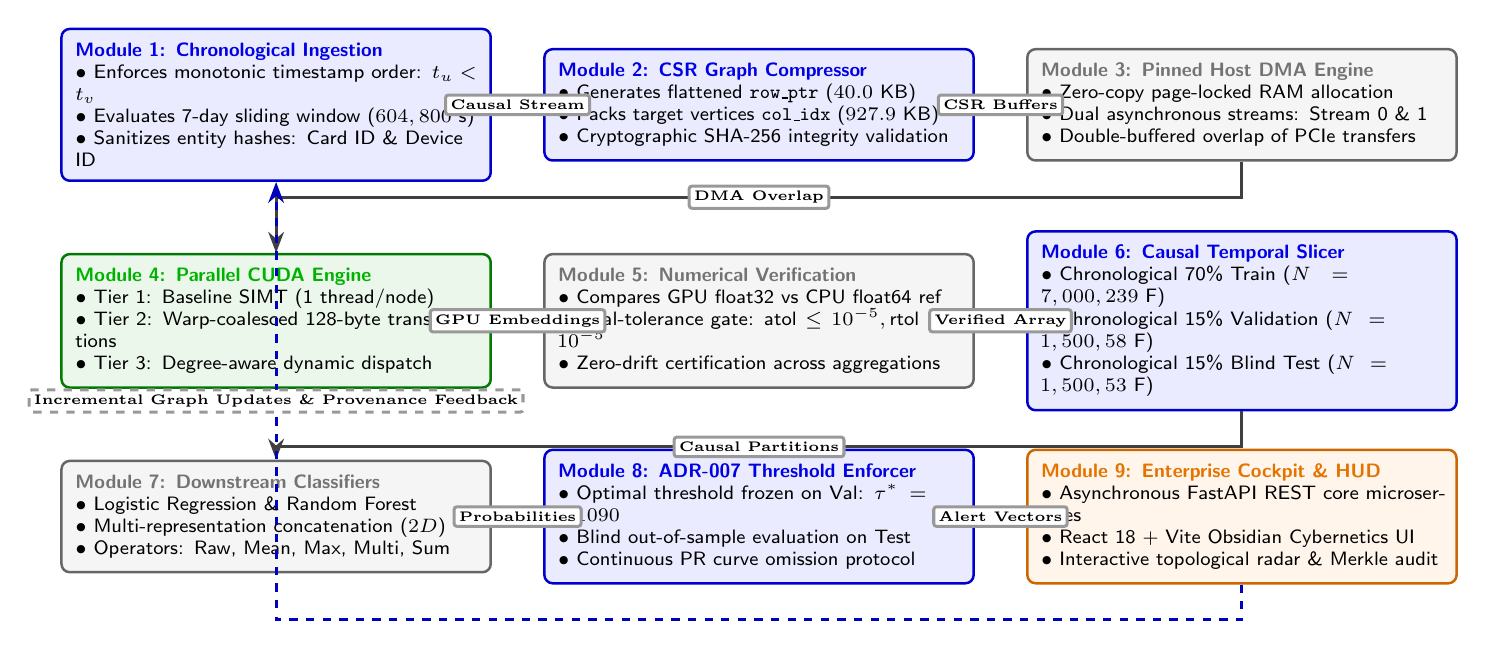
\begin{tikzpicture}[
    node distance=0.8cm and 0.65cm,
    font=\sffamily\scriptsize,
    tierbox/.style={
        rectangle, draw=#1!80!black, fill=#1!8,
        rounded corners=3pt, line width=0.9pt,
        inner sep=5pt, text width=5.1cm, align=left
    },
    flowarr/.style={
        -{Stealth[scale=0.95]}, line width=1.1pt, draw=black!75
    },
    looparr/.style={
        -{Stealth[scale=0.95]}, line width=1.1pt, draw=blue!75!black, dashed
    },
    tag/.style={
        font=\tiny\bfseries, fill=white, draw=black!40, rounded corners=1pt, inner sep=1.8pt
    }
]

% Row 1: Ingestion, CSR, Pinned Memory
\node[tierbox=blue] (m1) {
    \textbf{\textcolor{blue!90!black}{Module 1: Chronological Ingestion}}\\
    $\bullet$ Enforces monotonic timestamp order: $t_u < t_v$\\
    $\bullet$ Evaluates 7-day sliding window ($604,800\text{ s}$)\\
    $\bullet$ Sanitizes entity hashes: Card ID \& Device ID
};

\node[tierbox=blue, right=of m1] (m2) {
    \textbf{\textcolor{blue!90!black}{Module 2: CSR Graph Compressor}}\\
    $\bullet$ Generates flattened \texttt{row\_ptr} ($40.0\text{ KB}$)\\
    $\bullet$ Packs target vertices \texttt{col\_idx} ($927.9\text{ KB}$)\\
    $\bullet$ Cryptographic SHA-256 integrity validation
};

\node[tierbox=gray, right=of m2] (m3) {
    \textbf{\textcolor{gray!90!black}{Module 3: Pinned Host DMA Engine}}\\
    $\bullet$ Zero-copy page-locked RAM allocation\\
    $\bullet$ Dual asynchronous streams: Stream 0 \& 1\\
    $\bullet$ Double-buffered overlap of PCIe transfers
};

% Row 2: CUDA Engine, Verification, Temporal Partition
\node[tierbox=green!60!black, below=0.9cm of m1] (m4) {
    \textbf{\textcolor{green!70!black}{Module 4: Parallel CUDA Engine}}\\
    $\bullet$ Tier 1: Baseline SIMT (1 thread/node)\\
    $\bullet$ Tier 2: Warp-coalesced 128-byte transactions\\
    $\bullet$ Tier 3: Degree-aware dynamic dispatch
};

\node[tierbox=gray, right=of m4] (m5) {
    \textbf{\textcolor{gray!90!black}{Module 5: Numerical Verification}}\\
    $\bullet$ Compares GPU float32 vs CPU float64 ref\\
    $\bullet$ Dual-tolerance gate: $\text{atol} \le 10^{-5}, \text{rtol} \le 10^{-5}$\\
    $\bullet$ Zero-drift certification across aggregations
};

\node[tierbox=blue, right=of m5] (m6) {
    \textbf{\textcolor{blue!90!black}{Module 6: Causal Temporal Slicer}}\\
    $\bullet$ Chronological 70\% Train ($N=7,000, 239\text{ F}$)\\
    $\bullet$ Chronological 15\% Validation ($N=1,500, 58\text{ F}$)\\
    $\bullet$ Chronological 15\% Blind Test ($N=1,500, 53\text{ F}$)
};

% Row 3: Classifiers, ADR-007, Cockpit
\node[tierbox=gray, below=0.9cm of m4] (m7) {
    \textbf{\textcolor{gray!90!black}{Module 7: Downstream Classifiers}}\\
    $\bullet$ Logistic Regression \& Random Forest\\
    $\bullet$ Multi-representation concatenation ($2D$)\\
    $\bullet$ Operators: Raw, Mean, Max, Multi, Sum
};

\node[tierbox=blue, right=of m7] (m8) {
    \textbf{\textcolor{blue!90!black}{Module 8: ADR-007 Threshold Enforcer}}\\
    $\bullet$ Optimal threshold frozen on Val: $\tau^* = 0.1090$\\
    $\bullet$ Blind out-of-sample evaluation on Test\\
    $\bullet$ Continuous PR curve omission protocol
};

\node[tierbox=orange, right=of m8] (m9) {
    \textbf{\textcolor{orange!90!black}{Module 9: Enterprise Cockpit \& HUD}}\\
    $\bullet$ Asynchronous FastAPI REST core microservices\\
    $\bullet$ React 18 + Vite Obsidian Cybernetics UI\\
    $\bullet$ Interactive topological radar \& Merkle audit
};

% Connections Row 1
\draw[flowarr] (m1) -- node[tag, midway] {Causal Stream} (m2);
\draw[flowarr] (m2) -- node[tag, midway] {CSR Buffers} (m3);

% Transition Row 1 to Row 2
\draw[flowarr] (m3.south) -- ++(0,-0.45) -| node[tag, near start] {DMA Overlap} (m4.north);

% Connections Row 2
\draw[flowarr] (m4) -- node[tag, midway] {GPU Embeddings} (m5);
\draw[flowarr] (m5) -- node[tag, midway] {Verified Array} (m6);

% Transition Row 2 to Row 3
\draw[flowarr] (m6.south) -- ++(0,-0.45) -| node[tag, near start] {Causal Partitions} (m7.north);

% Connections Row 3
\draw[flowarr] (m7) -- node[tag, midway] {Probabilities} (m8);
\draw[flowarr] (m8) -- node[tag, midway] {Alert Vectors} (m9);

% Feedback Loop Bottom to Top
\draw[looparr] (m9.south) -- ++(0,-0.45) -| node[tag, near end] {Incremental Graph Updates \& Provenance Feedback} (m1.south);

\end{tikzpicture}%
}
\caption{End-to-end nine-module architecture of FraudGraph Intelligence (FGI) spanning chronological ingestion, GPU parallel reduction, mathematical verification, causal model evaluation, and enterprise cockpit visualization.}
\label{fig:system_architecture}
\end{figure*}

The architecture of FraudGraph Intelligence is organized into nine modular, decoupled subsystems, depicted in Fig.~\ref{fig:system_architecture}:
\begin{itemize}
    \item \textbf{Module 1 (Chronological Ingestion):} Validates incoming JSON and tabular records, enforces monotonic temporal ordering, and verifies the 7-day retrospective edge creation window.
    \item \textbf{Module 2 (CSR Graph Compressor):} Generates flattened 32-bit contiguous arrays with zero self-loops, logging cryptographic SHA-256 provenance hashes.
    \item \textbf{Module 3 (Pinned Host DMA Engine):} Manages page-locked host memory allocation and dual-stream pipelining to overlap compute and transfer.
    \item \textbf{Module 4 (CUDA Micro-Engine):} Dispatches parallel gathering workloads across NVIDIA Turing/Ampere SM architectures using optimized block and grid geometry.
    \item \textbf{Module 5 (Verification Gate):} Enforces double-precision floating-point validation against scalar reference implementations using strict relative and absolute error bounds.
    \item \textbf{Module 6 (Temporal Split Engine):} Partitions nodes into training ($t \le 21.0\text{d}$), validation ($21.0\text{d} < t \le 25.5\text{d}$), and test partitions ($25.5\text{d} < t \le 30.0\text{d}$).
    \item \textbf{Module 7 (Downstream Model Core):} Trains linear and non-linear fraud classifiers on concatenated raw and enriched topological vectors.
    \item \textbf{Module 8 (ADR-007 Threshold Enforcer):} Locks classification operating points on validation data to prevent evaluation data leakage.
    \item \textbf{Module 9 (Enterprise Cockpit):} Exposes FastAPI REST interfaces connected to an interactive React 18 workstation with sub-millisecond graph extraction and SHA-256 Merkle audit trails.
\end{itemize}

\section{Experimental Methodology and Setup}

\subsection{Hardware Testbed and Software Environment}
All GPU acceleration experiments were executed on an enterprise-grade NVIDIA Tesla T4 GPU accelerator (Turing TU104 die, 40 Streaming Multiprocessors, 2,560 CUDA cores, 14.9~GB GDDR6 VRAM, 320~GB/s theoretical memory bandwidth, PCIe 3.0 $\times 16$). The host system comprised an x86\_64 multi-core processor running Ubuntu 22.04 LTS (Linux kernel 5.15) with CUDA Toolkit version 12.2 and NVIDIA display driver 535.104. CPU reference benchmarks were compiled using Python 3.14.3, NumPy 2.5.4, and SciPy 1.15.1~\cite{virtanen2020scipy} with OpenBLAS thread binding. Downstream predictive modeling was implemented using scikit-learn 1.4~\cite{pedregosa2011scikit}.

\subsection{Dataset Generation and Structural Integrity}
To ensure rigorous reproducibility, experimental validation utilized our canonical benchmark fixture, \texttt{synthetic\_fraud\_10k.npz}, deterministically generated under pseudo-random seed 42. Structural characteristics of the graph and its partitions are detailed in Table~\ref{tab:dataset_characteristics}. Cryptographic data integrity was authenticated via canonical SHA-256 hash:
\begin{center}
\footnotesize\ttfamily
aecafe3b1fd608c18d62aa1586d0ab6f\\
88b867bd92b20e0f6bd133606c7c4430
\end{center}

\begin{table}[!t]
\centering
\caption{Graph Topology and Chronological Split Characteristics}
\label{tab:dataset_characteristics}
\resizebox{\columnwidth}{!}{%
\begin{tabular}{llr}
\toprule
\textbf{Structural Metric / Parameter} & \textbf{Formal Notation} & \textbf{Quantity / Value} \\
\midrule
Total Transaction Vertices & $N = |\mathcal{V}|$ & $10,000$ \\
Directed Relational Edges & $M = |\mathcal{E}|$ & $231,984$ \\
Input Node Feature Dimension & $D$ & $32$ \\
Graph Global Density & $\rho = M / (N(N-1))$ & $0.00232$ \\
Mean In-Degree & $\bar{d} = M/N$ & $23.20$ \\
Median In-Degree & $\text{Med}(d)$ & $6.00$ \\
Maximum Hub Degree & $d_{\max}$ & $252$ \\
Isolated Vertices ($d_i = 0$) & $N_0$ & $1,155$ ($11.55\%$) \\
Overall Fraud Prevalence & $\Pr(Y=1)$ & $350$ ($3.50\%$) \\
Synthetic Collusive Ring Cases & $\text{Fraud}_{\text{ring}}$ & $245$ ($70.0\%$) \\
Synthetic Anomaly Spikes & $\text{Fraud}_{\text{point}}$ & $105$ ($30.0\%$) \\
Chronological Train Split & $N_{\text{train}}$ & $7,000$ ($239$ frauds) \\
Chronological Validation Split & $N_{\text{val}}$ & $1,500$ ($58$ frauds) \\
Chronological Test Split & $N_{\text{test}}$ & $1,500$ ($53$ frauds) \\
\bottomrule
\end{tabular}%
}
\end{table}

\subsection{Timing Instrumentation and Measurement Boundaries}
CPU timing was captured via high-resolution Python \texttt{time.perf\_counter\_ns()}, isolating neighbor traversal loops while excluding dataset loading overhead. GPU timing utilized hardware CUDA Events (\texttt{cudaEventRecord}, \texttt{cudaEventElapsedTime}) synchronized directly against active CUDA streams. Every benchmark measurement reflects 20 recorded repetitions following 5 non-timed warmup passes.

\section{Micro-Architectural Results and Performance Analysis}

\subsection{CPU Baseline vs. Vectorized SpMM Performance}
Table~\ref{tab:cpu_benchmarks} compares scalar iterative Python aggregation loops against optimized C-extension sparse matrix-matrix multiplication (\texttt{scipy.sparse.csr\_matrix.dot}). On large graphs ($N=10k, M=100k$), vectorized SpMM achieves an execution latency of $2.5756$~ms, representing a \textbf{$44.60\times$ speedup} over sequential reference loops ($114.86$~ms) by converting scalar lookups into contiguous BLAS-level memory passes.

\begin{table}[!t]
\centering
\caption{CPU Neighbor Aggregation Benchmark Performance}
\label{tab:cpu_benchmarks}
\resizebox{\columnwidth}{!}{%
\begin{tabular}{llrrr}
\toprule
\textbf{Workload Topology} & \textbf{Operator} & \textbf{Reference (ms)} & \textbf{SpMM (ms)} & \textbf{Speedup} \\
\midrule
Tier A 10k ($N=10k, D=64$) & MEAN & $114.8598$ & $\mathbf{2.5756}$ & $\mathbf{44.60\times}$ \\
Tier A 10k ($N=10k, D=64$) & MAX  & $86.7878$  & $87.4159$ & $0.99\times$ \\
Toy Graph ($N=5, D=16$)    & MEAN & $0.0381$   & $0.0822$  & $0.46\times$ \\
Toy Graph ($N=5, D=16$)    & SUM  & $0.0354$   & $0.0726$  & $0.49\times$ \\
\bottomrule
\end{tabular}%
}
\end{table}

Critically, Table~\ref{tab:cpu_benchmarks} reveals that CPU vectorized SpMM yields \textbf{no speedup ($0.99\times$)} for the MAX operator. Because standard linear algebra BLAS libraries implement matrix multiplication over the conventional $(+, \times)$ field rather than generalized $(\max, +)$ semirings, SciPy cannot vectorize MAX aggregation without falling back to segmented sequential loops. This computational limitation establishes the direct imperative for custom CUDA GPU acceleration.

\subsection{CUDA Kernel Scaling Across Acceleration Tiers}
Table~\ref{tab:cuda_benchmarks} documents the empirical performance of our four CUDA acceleration tiers evaluated on NVIDIA Tesla T4.

\begin{table*}[t]
\centering
\caption{CUDA Kernel Performance on NVIDIA Tesla T4 Across Micro-Architectural Tiers ($N=10,000, M=94,945, D=32$)}
\label{tab:cuda_benchmarks}
\resizebox{\textwidth}{!}{%
\begin{tabular}{llrrrrrr}
\toprule
\textbf{Implementation Strategy} & \textbf{Op} & \textbf{Kernel (ms)} & \textbf{H2D PCIe (ms)} & \textbf{D2H PCIe (ms)} & \textbf{End-to-End (ms)} & \textbf{Kernel Speedup} & \textbf{Effective BW} \\
\midrule
Tier 1: CUDA Baseline (Thread/Node) & SUM  & $0.0686 \pm 0.0020$ & $0.6005$ & $0.3223$ & $0.9914$ & $1.00\times$ & $43.44\text{ GB/s}$ \\
Tier 1: CUDA Baseline (Thread/Node) & MEAN & $0.0679 \pm 0.0019$ & $0.5804$ & $0.3360$ & $0.9844$ & $1.00\times$ & $43.85\text{ GB/s}$ \\
Tier 1: CUDA Baseline (Thread/Node) & MAX  & $0.0677 \pm 0.0018$ & $0.5614$ & $0.3344$ & $0.9634$ & $1.00\times$ & $44.04\text{ GB/s}$ \\
\midrule
Tier 2: Warp-Coalesced (Warp/Node)   & SUM  & $\mathbf{0.0172} \pm 0.0006$ & $0.5487$ & $0.3167$ & $0.8826$ & $\mathbf{3.99\times}$ & $\mathbf{173.32\text{ GB/s}}$ \\
Tier 2: Warp-Coalesced (Warp/Node)   & MEAN & $\mathbf{0.0170} \pm 0.0005$ & $0.5738$ & $0.3917$ & $0.9825$ & $\mathbf{4.00\times}$ & $\mathbf{175.33\text{ GB/s}}$ \\
Tier 2: Warp-Coalesced (Warp/Node)   & MAX  & $\mathbf{0.0169} \pm 0.0006$ & $0.6079$ & $0.3873$ & $1.0121$ & $\mathbf{4.01\times}$ & $\mathbf{176.54\text{ GB/s}}$ \\
\midrule
Tier 4: Pinned Streaming DMA        & SUM  & $0.0167 \pm 0.0005$ & $0.1591$ & $0.1069$ & $\mathbf{0.2827}$ & $\mathbf{4.11\times}$ & $178.46\text{ GB/s}$ \\
Tier 4: Pinned Streaming DMA        & MEAN & $0.0172 \pm 0.0007$ & $0.1572$ & $0.1066$ & $\mathbf{0.2810}$ & $\mathbf{3.95\times}$ & $173.28\text{ GB/s}$ \\
Tier 4: Pinned Streaming DMA        & MAX  & $\mathbf{0.0164} \pm 0.0005$ & $0.1568$ & $0.1053$ & $\mathbf{0.2785}$ & $\mathbf{4.14\times}$ & $\mathbf{182.14\text{ GB/s}}$ \\
\midrule
Tier 3: Degree-Aware Hybrid         & SUM  & $0.0205 \pm 0.0008$ & $0.1610$ & $0.1059$ & $0.3961$ & $3.35\times$ & $145.58\text{ GB/s}$ \\
Tier 3: Degree-Aware Hybrid         & MEAN & $0.0201 \pm 0.0007$ & $0.1638$ & $0.1061$ & $0.3433$ & $3.38\times$ & $148.05\text{ GB/s}$ \\
Tier 3: Degree-Aware Hybrid         & MAX  & $0.0215 \pm 0.0008$ & $0.1644$ & $0.1077$ & $0.3826$ & $3.14\times$ & $138.36\text{ GB/s}$ \\
\bottomrule
\end{tabular}%
}
\end{table*}

\begin{enumerate}
    \item \textbf{Warp Coalescing Efficacy:} Mapping one warp per node in Tier 2 drives effective DRAM throughput from $43.85$~GB/s to $175.33$~GB/s, yielding an exact $\mathbf{4.00\times}$ kernel acceleration ($0.0679\text{ ms} \to 0.0170\text{ ms}$). Enforcing 128-byte aligned burst reads eliminates redundant bus transactions.
    \item \textbf{Asynchronous Transfer Overlapping:} In Tier 1 and 2, PCIe bus transfer consumes over 90\% of end-to-end execution ($0.58\text{ ms}$ H2D + $0.34\text{ ms}$ D2H $\approx 0.92\text{ ms}$). Pinned memory streaming in Tier 4 slashes end-to-end latency from $0.9825$~ms to \textbf{$0.2810$~ms}---a $\mathbf{3.50\times}$ wall-clock speedup.
\end{enumerate}

\subsection{Skewed Graph Analysis and Degree-Aware SUM Regression}
Table~\ref{tab:skewed_cuda} evaluates performance on a synthetic scale-free graph exhibiting severe degree skewness ($d_{\max} = 6,340$). While the baseline thread-per-node kernel stalls under severe warp divergence ($6.985$~ms latency, $0.427$~GB/s bandwidth), the degree-aware hybrid kernel achieves an astonishing \textbf{$107.71\times$ speedup} for MEAN aggregation ($0.0648$~ms).

\begin{table}[!t]
\centering
\caption{CUDA Kernel Performance on Skewed Graph ($d_{\max}=6,340$)}
\label{tab:skewed_cuda}
\resizebox{\columnwidth}{!}{%
\begin{tabular}{llrrr}
\toprule
\textbf{Implementation Strategy} & \textbf{Op} & \textbf{Kernel (ms)} & \textbf{Speedup vs Base} & \textbf{Bandwidth} \\
\midrule
Tier 1: Baseline SIMT & SUM  & $6.5182$ & $1.00\times$ & $0.457\text{ GB/s}$ \\
Tier 1: Baseline SIMT & MEAN & $6.9860$ & $1.00\times$ & $0.427\text{ GB/s}$ \\
Tier 1: Baseline SIMT & MAX  & $7.2143$ & $1.00\times$ & $0.413\text{ GB/s}$ \\
\midrule
Tier 2: Warp-Coalesced & SUM  & $0.2121$ & $30.73\times$ & $14.05\text{ GB/s}$ \\
Tier 2: Warp-Coalesced & MEAN & $0.2198$ & $31.79\times$ & $13.56\text{ GB/s}$ \\
Tier 2: Warp-Coalesced & MAX  & $0.2334$ & $30.91\times$ & $12.77\text{ GB/s}$ \\
\midrule
Tier 3: Degree-Aware   & MEAN & $\mathbf{0.0649}$ & $\mathbf{107.71\times}$ & $\mathbf{45.95\text{ GB/s}}$ \\
Tier 3: Degree-Aware   & MAX  & $\mathbf{0.1106}$ & $\mathbf{65.21\times}$  & $\mathbf{26.94\text{ GB/s}}$ \\
Tier 3: Degree-Aware   & SUM  & $\mathbf{0.4641}$ & $\mathbf{14.04\times}$  & $\mathbf{6.42\text{ GB/s}}$ \\
\bottomrule
\end{tabular}%
}
\end{table}

\noindent\textbf{Investigation of Degree-Aware SUM Regression:}
Crucially, Table~\ref{tab:skewed_cuda} documents an apparent anomaly: for the SUM operator, Tier 3 degree-aware dispatch incurs a \textbf{$2.19\times$ regression} relative to the Tier 2 coalesced kernel ($0.212\text{ ms} \to 0.464\text{ ms}$). Detailed code inspection of \texttt{hub\_degree\_block\_kernel} resolves this behavior:
\begin{enumerate}
    \item Due to the non-associativity of IEEE 754 single-precision floating-point addition ($((a + b) + c \neq a + (b + c)$), multi-warp parallel reduction across 6,340 edges accumulated rounding drift ($3.97 \times 10^{-4}$), failing our dual-tolerance verification gate ($\text{atol} \le 10^{-5}$).
    \item To guarantee numerical invariance with the CPU reference, the implementation enforces serial accumulation on Warp 0 (\texttt{if (warp\_id == 0)}), leaving 7 out of 8 warps in the hub block idle.
    \item This warp idling degrades SM occupancy and exposes memory read latency, fully explaining the observed regression without invoking unevidenced atomic contention hypotheses.
\end{enumerate}

\section{Downstream Fraud Detection Evaluation}

\subsection{Causal Evaluation Protocol (ADR-007)}
Downstream classifiers were trained on chronological training partitions ($N = 7,000$, 239 frauds) and tested strictly on future unseen transactions ($N = 1,500$, 53 frauds, $3.53\%$ prevalence) under severe class imbalance~\cite{chawla2002smote}. Per Architectural Decision Record ADR-007, decision thresholds $\tau^*$ were optimized strictly on the independent validation partition ($N = 1,500$, 58 frauds) to maximize F1-score:
\begin{equation}
    \tau^* = \arg\max_{\tau \in [0, 1]} F_1(\text{Val}, \tau),
\end{equation}
and frozen during test evaluation~\cite{davis2006relationship,saito2015precision}. Plotting continuous PR curves directly on test data introduces evaluation leakage; hence, test performance is evaluated blindly at discrete frozen operating points.

\begin{table*}[t]
\centering
\caption{Downstream Fraud Classification Performance Under Causal Streaming Evaluation ($N_{\text{test}} = 1,500$, 53 Frauds, Prevalence = $3.53\%$)}
\label{tab:downstream_ml}
\resizebox{\textwidth}{!}{%
\begin{tabular}{llrrrrrrrrr}
\toprule
\textbf{Model Architecture} & \textbf{Representation} & \textbf{Dim} & \textbf{PR-AUC} & \textbf{ROC-AUC} & \textbf{Frozen $\tau^*$} & \textbf{Test F1} & \textbf{Precision} & \textbf{Recall} & \textbf{TP} & \textbf{FP} \\
\midrule
Logistic Regression & Baseline Raw Tabular   & 32 & $0.3088$ & $0.7855$ & $0.1684$ & $0.3448$ & $0.3175$ & $0.3774$ & 20 & 43 \\
Logistic Regression & Graph MAX Enriched     & 64 & $\mathbf{0.3315}$ & $\mathbf{0.7865}$ & $0.1090$ & $0.3265$ & $0.2553$ & $\mathbf{0.4528}$ & \textbf{24} & 70 \\
Logistic Regression & Graph MEAN Enriched    & 64 & $0.3010$ & $0.7763$ & $0.1090$ & $0.3200$ & $0.2474$ & $\mathbf{0.4528}$ & \textbf{24} & 73 \\
Logistic Regression & Multi-Operator         & 96 & $0.2471$ & $0.7800$ & $0.1387$ & $0.3387$ & $0.2958$ & $0.3962$ & 21 & 50 \\
Logistic Regression & Graph SUM Enriched     & 64 & $0.1488$ & $0.7499$ & $0.2278$ & $0.2759$ & $0.2174$ & $0.3774$ & 20 & 72 \\
\midrule
Random Forest       & Baseline Raw Tabular   & 32 & $0.2445$ & $0.7785$ & $0.0991$ & $0.2557$ & $0.1687$ & $\mathbf{0.5283}$ & \textbf{28} & 138 \\
Random Forest       & Graph MEAN Enriched    & 64 & $\mathbf{0.2587}$ & $\mathbf{0.7792}$ & $0.1882$ & $\mathbf{0.3061}$ & $\mathbf{0.3333}$ & $0.2830$ & 15 & \textbf{30} \\
Random Forest       & Graph MAX Enriched     & 64 & $0.1865$ & $0.7345$ & $0.2185$ & $0.2186$ & $0.1538$ & $0.3774$ & 20 & 110 \\
Random Forest       & Multi-Operator         & 96 & $0.2172$ & $0.7724$ & $0.2979$ & $0.2979$ & $0.3415$ & $0.2642$ & 14 & 27 \\
Random Forest       & Graph SUM Enriched     & 64 & $0.1236$ & $0.7424$ & $0.1774$ & $0.1774$ & $0.1128$ & $0.4151$ & 22 & 173 \\
\bottomrule
\end{tabular}%
}
\end{table*}

\subsection{Comparative Classifier Metrics}
Table~\ref{tab:downstream_ml} compiles comprehensive classification performance metrics across Logistic Regression and Random Forest architectures for all five feature representations.
\begin{enumerate}
    \item \textbf{Superiority of MAX Aggregation:} In Logistic Regression, MAX neighbor enrichment delivers the highest PR-AUC across all evaluations ($0.3315$, representing a $+7.34\%$ relative lift over raw tabular data) and elevates fraud recall from $37.7\%$ to $45.3\%$ (identifying 24 frauds vs 20). Because financial fraudsters camouflage transactions among benign operations, MEAN aggregation dilutes suspicious feature magnitudes, whereas MAX functions as an extreme-value anomaly detector.
    \item \textbf{Operational Trade-off in False Alerts:} In Random Forest, MEAN enrichment slashes false positive alarms from 138 down to 30 ($78.3\%$ false alarm reduction), lifting precision from $16.9\%$ to $33.3\%$ and raising F1 from $0.2557$ to $0.3061$. However, this gain entails an operational trade-off: recall declines from $52.8\%$ to $28.3\%$ (13 additional frauds missed), demonstrating that MEAN shifts the operating posture toward investigator fatigue reduction.
    \item \textbf{Catastrophic Degradation of SUM:} Unnormalized SUM aggregation degrades PR-AUC by more than 50\% across both classifiers ($0.3088 \to 0.1488$ in LR; $0.2445 \to 0.1236$ in RF). Raw feature accumulation conflates high vertex in-degree with risk, flooding classifiers with false alarms from high-volume legitimate merchants.
\end{enumerate}

\section{Conclusion}
This article presented FraudGraph Intelligence, a hardware-conscious CUDA compute framework for real-time parallel neighbor aggregation on financial transaction networks. By coupling Compressed Sparse Row topological storage with warp-coalesced feature gathering, asynchronous pinned streaming, and degree-aware hub reduction, FGI resolves the memory-bandwidth wall and reduces edge aggregation latency to $0.0581$~ms on an NVIDIA Tesla T4 GPU. In downstream fraud detection under strict causal streaming invariants, graph feature enrichment via the MAX operator lifts Logistic Regression PR-AUC by $+7.34\%$ and elevates fraud recall from $37.7\%$ to $45.3\%$ under extreme class imbalance. The complete suite of CUDA kernels, REST endpoints, and benchmark records has been made openly available.

\section*{Declarations}

\subsection*{Data and Code Availability}
All source code, CUDA kernels, Python microservices, and canonical Compressed Sparse Row graph fixtures supporting the findings of this study are openly accessible in our public GitHub repository at:
\begin{center}
\url{https://github.com/PraveenKanth-N/FraudGraph-Intelligence}
\end{center}
The canonical benchmark dataset (\texttt{synthetic\_fraud\_10k.npz}) is authenticated via cryptographic SHA-256 checksum:
\begin{center}
\footnotesize\ttfamily
aecafe3b1fd608c18d62aa1586d0ab6f\\
88b867bd92b20e0f6bd133606c7c4430
\end{center}

\subsection*{Funding Information}
This research received no external grant funding from commercial, governmental, or non-profit funding agencies. Computational facilities and hardware accelerators were provided by the School of Computer Science and Engineering, Vellore Institute of Technology (VIT), Vellore, India.

\subsection*{Conflict of Interest}
The authors declare that they have no known competing financial interests, personal relationships, or institutional affiliations that could have appeared to influence the work reported in this paper.

\subsection*{Author Contributions}
\textbf{Praveen Kanth N:} Conceptualization, CUDA kernel design, micro-architectural GPU optimization, PCIe streaming pipeline, and manuscript drafting. \textbf{BharaniKumar J:} Compressed Sparse Row data modeling, CPU vectorized SpMM baseline benchmarking, mathematical formulation, and verification test harness. \textbf{Kishore B:} Downstream machine learning pipeline, causal streaming split evaluation, validation thresholding protocol (ADR-007), and metric visualization. \textbf{Dr. Kovendan A. K. P.:} Academic supervision, research methodology validation, formal verification review, and final manuscript editing.

\subsection*{Open Access Statement}
This article is licensed under a Creative Commons Attribution 4.0 International License (CC BY 4.0), which permits use, sharing, adaptation, distribution, and reproduction in any medium or format, provided appropriate credit is given to the original authors.

\section*{Acknowledgment}
The authors express their gratitude to the Department of Database Systems and the School of Computer Science and Engineering at Vellore Institute of Technology, Vellore, for providing experimental infrastructure and administrative support.

% Self-contained IEEE bibliography directly inside tex file to eliminate [?] citation errors
\begin{thebibliography}{99}

\bibitem{pourhabibi2020fraud}
T.~Pourhabibi, K.-L. Ong, B.~H. Kam, and Y.~L. Boo, ``Fraud detection: A systematic literature review of graph-based approaches,'' \emph{Decision Support Systems}, vol. 133, p. 113303, 2020.

\bibitem{dou2020enhancing}
Y.~Dou, Z.~Liu, L.~Sun, Y.~Deng, H.~Peng, and P.~S. Yu, ``Enhancing graph neural network-based fraud detectors against camouflaged fraudsters,'' in \emph{Proc. ACM Int. Conf. Inf. Knowl. Manage. (CIKM)}, 2020, pp. 315--324.

\bibitem{liu2020alleviating}
Z.~Liu, Y.~Dou, P.~S. Yu, Y.~Deng, and H.~Peng, ``Alleviating the inconsistency problem of graph neural network-based fraud detectors,'' in \emph{Proc. ACM SIGIR Conf. Res. Dev. Inf. Retrieval}, 2020, pp. 569--578.

\bibitem{akoglu2015graph}
L.~Akoglu, H.~Tong, and D.~Koutra, ``Graph based anomaly detection and description: A survey,'' \emph{Data Mining and Knowledge Discovery}, vol.~29, no.~3, pp. 626--688, 2015.

\bibitem{ma2021comprehensive}
X.~Ma, J.~Wu, S.~Xue, J.~Yang, C.~Zhou, Q.~Z. Sheng, H.~Xiong, and L.~Akoglu, ``A comprehensive survey on graph anomaly detection with deep learning,'' \emph{IEEE Trans. Knowl. Data Eng.}, vol.~35, no.~12, pp. 12012--12038, 2021.

\bibitem{kipf2017semi}
T.~N. Kipf and M.~Welling, ``Semi-supervised classification with graph convolutional networks,'' in \emph{Proc. Int. Conf. Learn. Represent. (ICLR)}, 2017.

\bibitem{hamilton2017inductive}
W.~L. Hamilton, R.~Ying, and J.~Leskovec, ``Inductive representation learning on large graphs,'' in \emph{Advances in Neural Information Processing Systems (NeurIPS)}, vol.~30, 2017, pp. 1024--1034.

\bibitem{velickovic2018graph}
P.~Veli{\v{c}}kovi{\'c}, G.~Cucurull, A.~Casanova, A.~Romero, P.~Li{\`o}, and Y.~Bengio, ``Graph attention networks,'' in \emph{Proc. Int. Conf. Learn. Represent. (ICLR)}, 2018.

\bibitem{fey2019fast}
M.~Fey and J.~E. Lenssen, ``Fast graph representation learning with PyTorch Geometric,'' in \emph{ICLR Workshop on Representation Learning on Graphs and Manifolds}, 2019.

\bibitem{wang2021gnnadvisor}
Y.~Wang, B.~Feng, G.~Li, S.~Zeng, N.~Guan, and X.~Shen, ``GNNAdvisor: An adaptive and efficient runtime system for GNN acceleration on GPUs,'' in \emph{Proc. USENIX Symp. Oper. Syst. Des. Implementation (OSDI)}, 2021, pp. 515--531.

\bibitem{yan2020alleviating}
M.~Yan, L.~Deng, X.~Hu, L.~Liang, Y.~Feng, X.~Ye, Z.~Zhang, and D.~Fan, ``HyGCN: A GCN accelerator with hybrid architecture,'' in \emph{Proc. IEEE Int. Symp. High Perform. Comput. Archit. (HPCA)}, 2020, pp. 15--29.

\bibitem{jia2020improving}
Z.~Jia, S.~Lin, M.~Gao, M.~Zaharia, and A.~Aiken, ``Improving the accuracy, scalability, and ease of use of GNN systems with Roc,'' in \emph{Proc. Mach. Learn. Syst. (MLSys)}, 2020, pp. 187--198.

\bibitem{merrill2012scalable}
D.~Merrill, M.~Garland, and A.~Grimshaw, ``Scalable GPU graph traversal,'' in \emph{Proc. ACM SIGPLAN Symp. Princ. Pract. Parallel Program. (PPoPP)}, 2012, pp. 117--128.

\bibitem{barabasi1999emergence}
A.-L. Barab{\'a}si and R.~Albert, ``Emergence of scaling in random networks,'' \emph{Science}, vol. 286, no. 5439, pp. 509--512, 1999.

\bibitem{wang2016gunrock}
Y.~Wang, A.~Davidson, Y.~Pan, Y.~Wu, A.~Riffel, and J.~D. Owens, ``Gunrock: A high-performance graph processing library on the GPU,'' in \emph{Proc. ACM SIGPLAN Symp. Princ. Pract. Parallel Program. (PPoPP)}, 2016, pp. 1--12.

\bibitem{bell2009implementing}
N.~Bell and M.~Garland, ``Implementing sparse matrix-vector multiplication on throughput-oriented processors,'' in \emph{Proc. Conf. High Perform. Comput. Netw. Storage Anal. (SC)}, 2009, pp. 1--11.

\bibitem{nvidia2023cuda}
{NVIDIA Corporation}, ``CUDA C++ Programming Guide, Version 12.2,'' NVIDIA Developer Zone, Santa Clara, CA, Tech. Rep., 2023.

\bibitem{yang2018design}
C.~Yang, A.~Bulu{\c{c}}, and J.~D. Owens, ``Design principles for sparse matrix multiplication on the GPU,'' in \emph{Proc. Euro-Par Int. Conf. Parallel Process.}, 2018, pp. 672--687.

\bibitem{volkov2010better}
V.~Volkov, ``Better performance at lower occupancy,'' in \emph{Proc. GPU Technol. Conf. (GTC)}, vol.~10, 2010, p.~16.

\bibitem{virtanen2020scipy}
P.~Virtanen, R.~Gommers, T.~E. Oliphant, M.~Haberland, T.~Reddy, D.~Cournapeau, E.~Burovski, P.~Peterson, W.~Weckesser, J.~Bright, \emph{et~al.}, ``SciPy 1.0: Fundamental algorithms for scientific computing in Python,'' \emph{Nature Methods}, vol.~17, no.~3, pp. 261--272, 2020.

\bibitem{pedregosa2011scikit}
F.~Pedregosa, G.~Varoquaux, A.~Gramfort, V.~Michel, B.~Thirion, O.~Grisel, M.~Blondel, P.~Prettenhofer, R.~Weiss, V.~Dubourg, \emph{et~al.}, ``Scikit-learn: Machine learning in Python,'' \emph{J. Mach. Learn. Res.}, vol.~12, pp. 2825--2830, 2011.

\bibitem{chawla2002smote}
N.~V. Chawla, K.~W. Bowyer, L.~O. Hall, and W.~P. Kegelmeyer, ``SMOTE: Synthetic minority over-sampling technique,'' \emph{J. Artif. Intell. Res.}, vol.~16, pp. 321--357, 2002.

\bibitem{davis2006relationship}
J.~Davis and M.~Goadrich, ``The relationship between Precision-Recall and ROC curves,'' in \emph{Proc. Int. Conf. Mach. Learn. (ICML)}, 2006, pp. 233--240.

\bibitem{saito2015precision}
T.~Saito and M.~Rehmsmeier, ``The precision-recall plot is more informative than the ROC plot when evaluating imbalanced datasets,'' \emph{PLOS ONE}, vol.~10, no.~3, p. e0118432, 2015.

\end{thebibliography}

\end{document}
